\documentclass{beamer}

\usepackage[croatian]{babel}
\usepackage[numbers, square]{natbib}
\usepackage[utf8]{inputenc}
\usepackage{courier}
\usepackage{listings}
\usepackage{mathtools}
\usepackage{relsize}

\newcommand{\engl}[1]{(engl.~\emph{#1})}
\setbeamertemplate{caption}[numbered]
\usetheme{Boadilla}

\renewcommand{\lstlistingname}{Isječak}
\DeclareMathOperator*{\argmax}{arg\,max}

\title[Završni rad br. 5709]{Sustav za određivanje strukture teksta na temelju položaja pojedinih znakova}
\author{Herman Zvonimir Došilović}
\institute[FER]{Sveučilište u Zagrebu\\ Fakultet elektrotehnike i računarstva}
\date{Zagreb, srpanj 2018.}
\logo{
\includegraphics[height=1.0cm]{images/logo.png}}

\begin{document}

\lstset{
    basicstyle=\linespread{1.2}\ttfamily\scriptsize,
    keepspaces=true,
    numbers=left,
    frame=single,
    showspaces=false,
    numberstyle=\ttfamily,
    columns=flexible,
    extendedchars=true,
    inputencoding=utf8,
    literate={®}{{\textregistered}}1,
    xleftmargin=.2\textwidth,
    xrightmargin=.2\textwidth,
}

\frame{\titlepage}

\begin{frame}
\frametitle{Sadržaj}
\tableofcontents
\end{frame}

\section{Uvod}
\subsection{Optičko raspoznavanje znakova}
\begin{frame}
\begin{itemize}
    \item Engl.~\textit{Optical Character Recognition} (\textit{OCR})
\end{itemize}
\frametitle{Uvod}
\framesubtitle{Optičko raspoznavanje znakova}
\begin{figure}[htb]
    \centering
    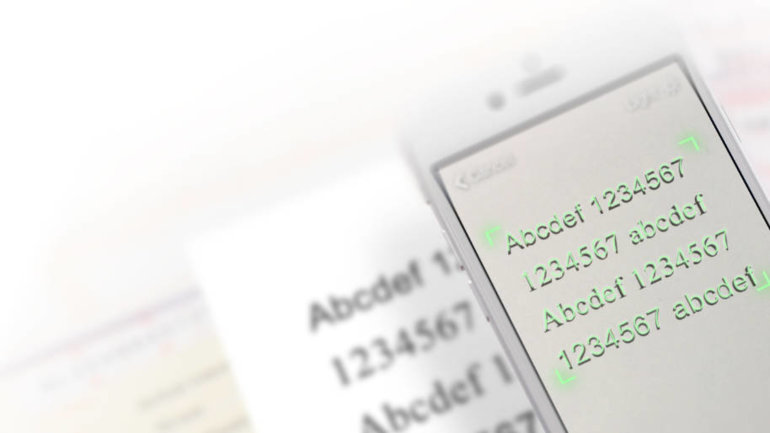
\includegraphics[width=10cm]{images/mobile-ocr.jpg}
    \caption{OCR-sustav na mobilnom uređaju. \citep{Microblink}}
    \label{fig:mobile-ocr}
\end{figure}
\end{frame}

\subsubsection{Primjene optičkog raspoznavanja znakova}
\begin{frame}
\frametitle{Optičko raspoznavanje znakova}
\framesubtitle{Primjene optičkog raspoznavanja znakova (1)}
\begin{itemize}
    \item Bankovne aplikacije za mobilne uređaje
    \begin{itemize}
        \item Plaćanje računa
        \item Otvaranje bankovnog računa (npr. Zagrebačka banka, Revolut, N26)
    \end{itemize}
    \item Turizam i hoteljerstvo
    \begin{itemize}
        \item Prijava boravka u hotelima
    \end{itemize}
    \item Registracija glasovanja na biralištima
    \item Registracija posjetitelja na raznim događajima
    \item Granične kontrole
    \item Upravljanje financijama
    \item Digitalizacija knjiga
    \item Detekcija znakova na registarskim pločicama
\end{itemize}
\end{frame}

\begin{frame}
\frametitle{Optičko raspoznavanje znakova}
\framesubtitle{Primjene optičkog raspoznavanja znakova (2)}
\begin{figure}[htb]
    \centering
    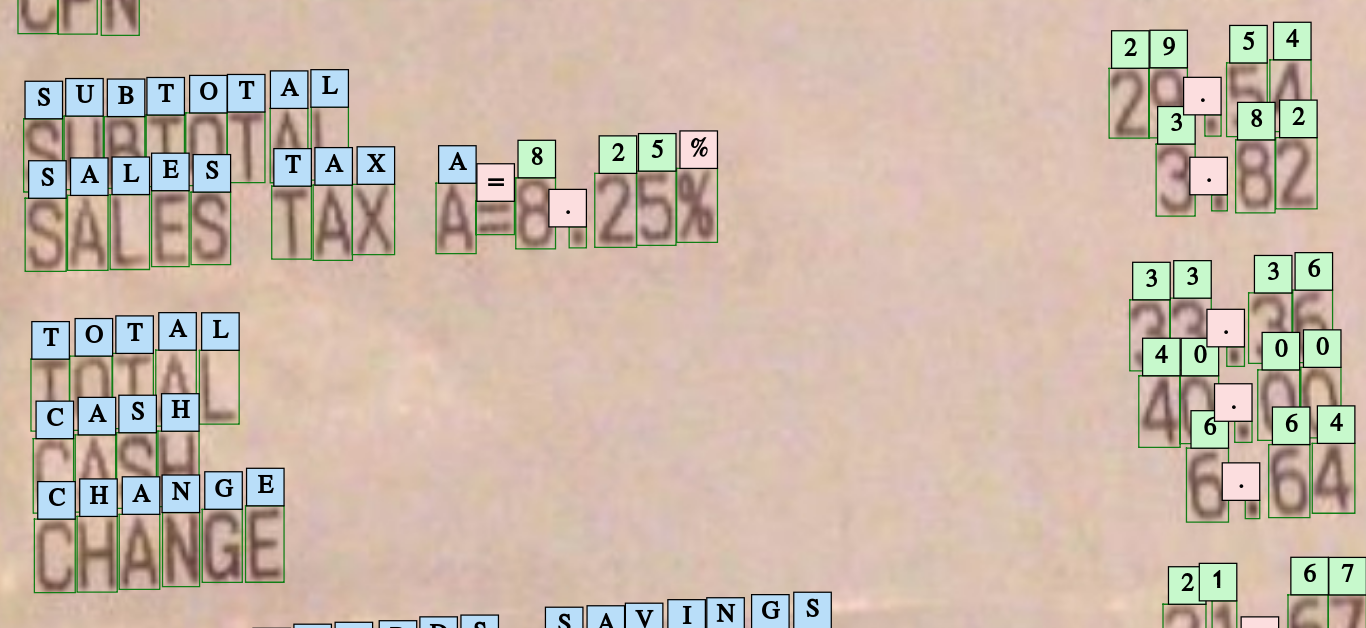
\includegraphics[width=12cm]{images/receipt-example-01.png}
    \caption{Vizualizacija rezultata OCR-sustava.}
    \label{fig:ocr-result-01}
\end{figure}
\end{frame}

\subsubsection{Komponente sustava za optičko raspoznavanje znakova}
\begin{frame}
\frametitle{Optičko raspoznavanje znakova}
\framesubtitle{Komponente sustava za optičko raspoznavanje znakova}
Optičko raspoznavanje znakova provodi se u nekoliko koraka:
\begin{itemize}
    \item pribavljanje slike,
    \item predobrada,
    \item segmentacija znakova,
    \item izdvajanje značajki znakova,
    \item klasifikacija znakova i
    \item \textbf{naknadna obrada}.
\end{itemize}
\end{frame}

\section{Određivanje strukture teksta na temelju položaja pojedinih znakova}
\subsection{Željena funkcionalnost}
\begin{frame}
\frametitle{Određivanje strukture teksta na temelju položaja pojedinih znakova}
\framesubtitle{Željena funkcionalnost}
\begin{figure}[htb]
    \centering
    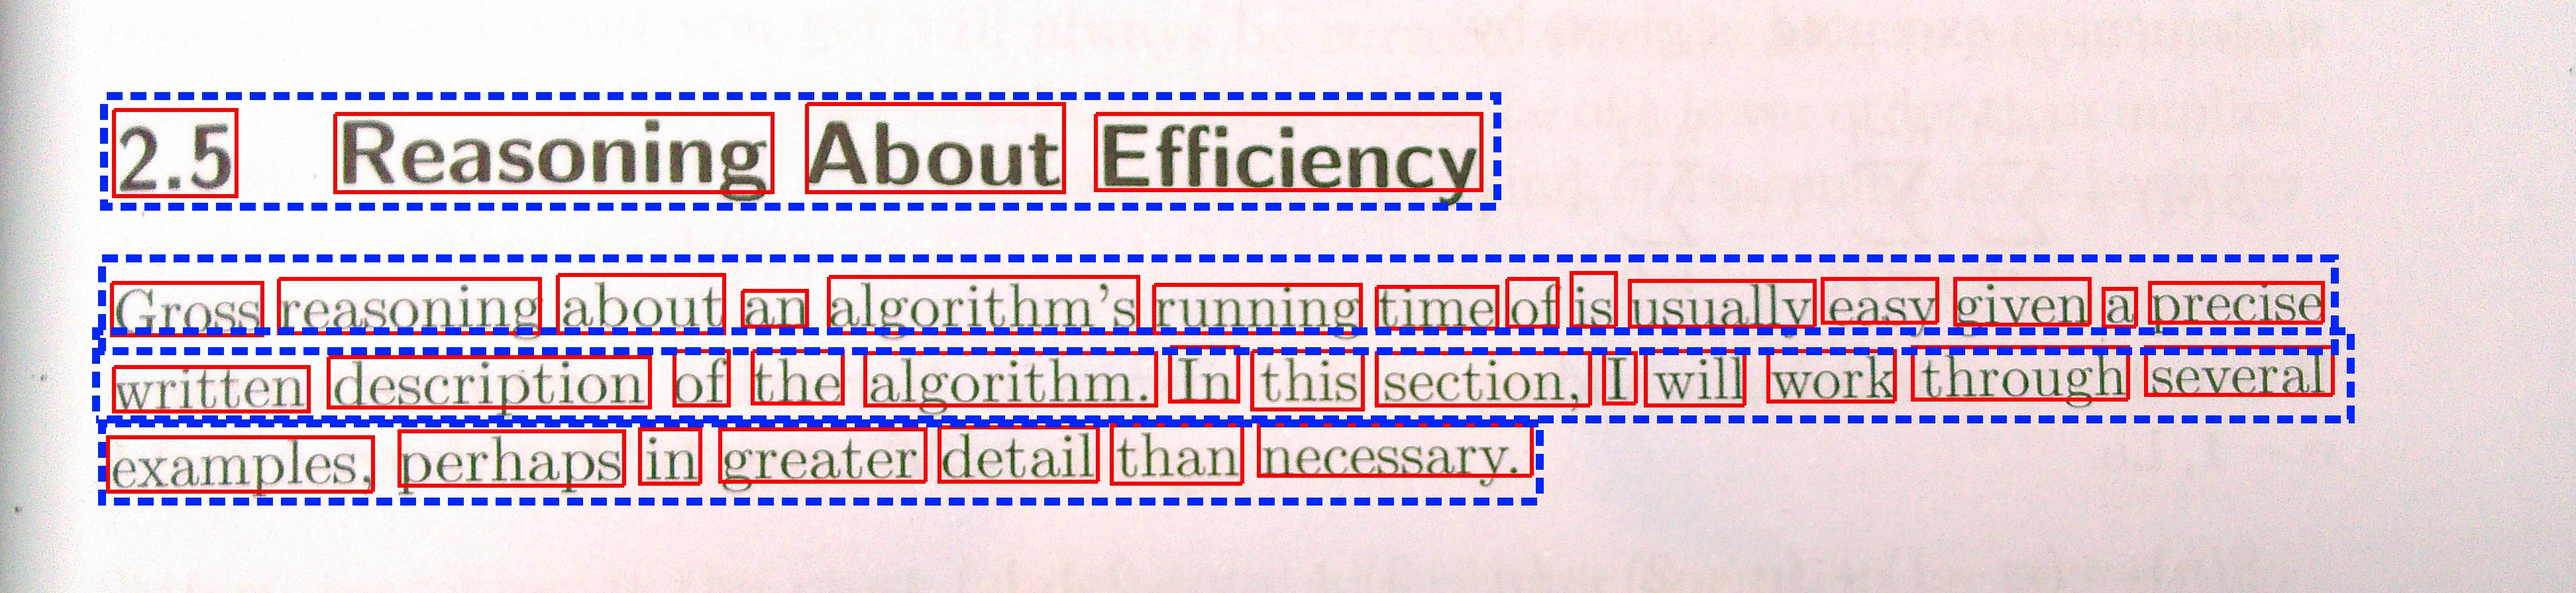
\includegraphics[width=\textwidth]{images/text-segmentation-01.jpg}
    \caption{Vizualizacija rezultata sustava za određivanje strukture teksta.}
    \label{fig:text-segmentation-01}
\end{figure}
\end{frame}

\subsection{Suradnja s OCR-sustavom}
\begin{frame}
\frametitle{Određivanje strukture teksta na temelju položaja pojedinih znakova}
\framesubtitle{Suradnja s OCR-sustavom}
\begin{figure}[htb]
    \centering
    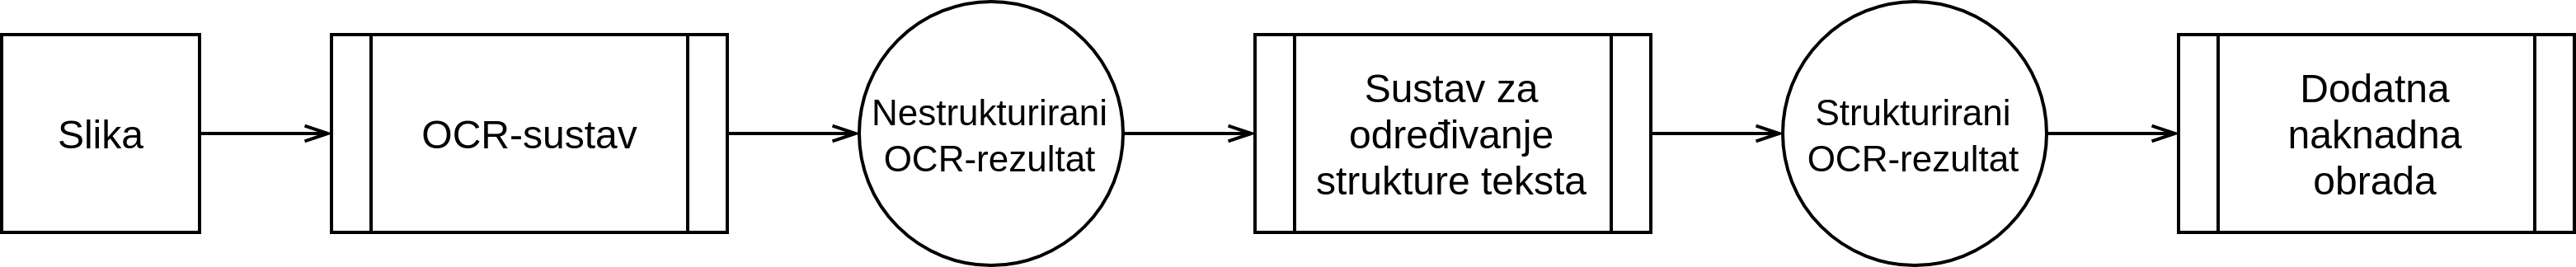
\includegraphics[width=\textwidth]{images/sustav-01.png}
    \caption{Suradnja OCR-sustava i sustava za određivanje strukture teksta.}
    \label{fig:sustav-01}
\end{figure}
\end{frame}

\subsection{Skup podataka za ispitivanje}
\begin{frame}
\frametitle{Određivanje strukture teksta na temelju položaja pojedinih znakova}
\framesubtitle{Skup podataka za ispitivanje}
Skup podataka za ispitivanje sastoji se od:
\begin{itemize}
    \item slika,
    \item ulaznih datoteka u formatu JSON i
    \item očekivanih izlaznih datoteka.
\end{itemize}
\end{frame}
\begin{frame}
\frametitle{Skup podataka za ispitivanje}
\framesubtitle{Slike (1)}
\begin{itemize}
    \item \textbf{Ručno} označene i klasificirane slike.
    \item 100 slika računa iz trgovina (ukupno 85068 znakova).
    \item 34 slike sadržaja iz knjiga (ukupno 25092 znaka).
\end{itemize}
\begin{figure}[htb]
    \centering
    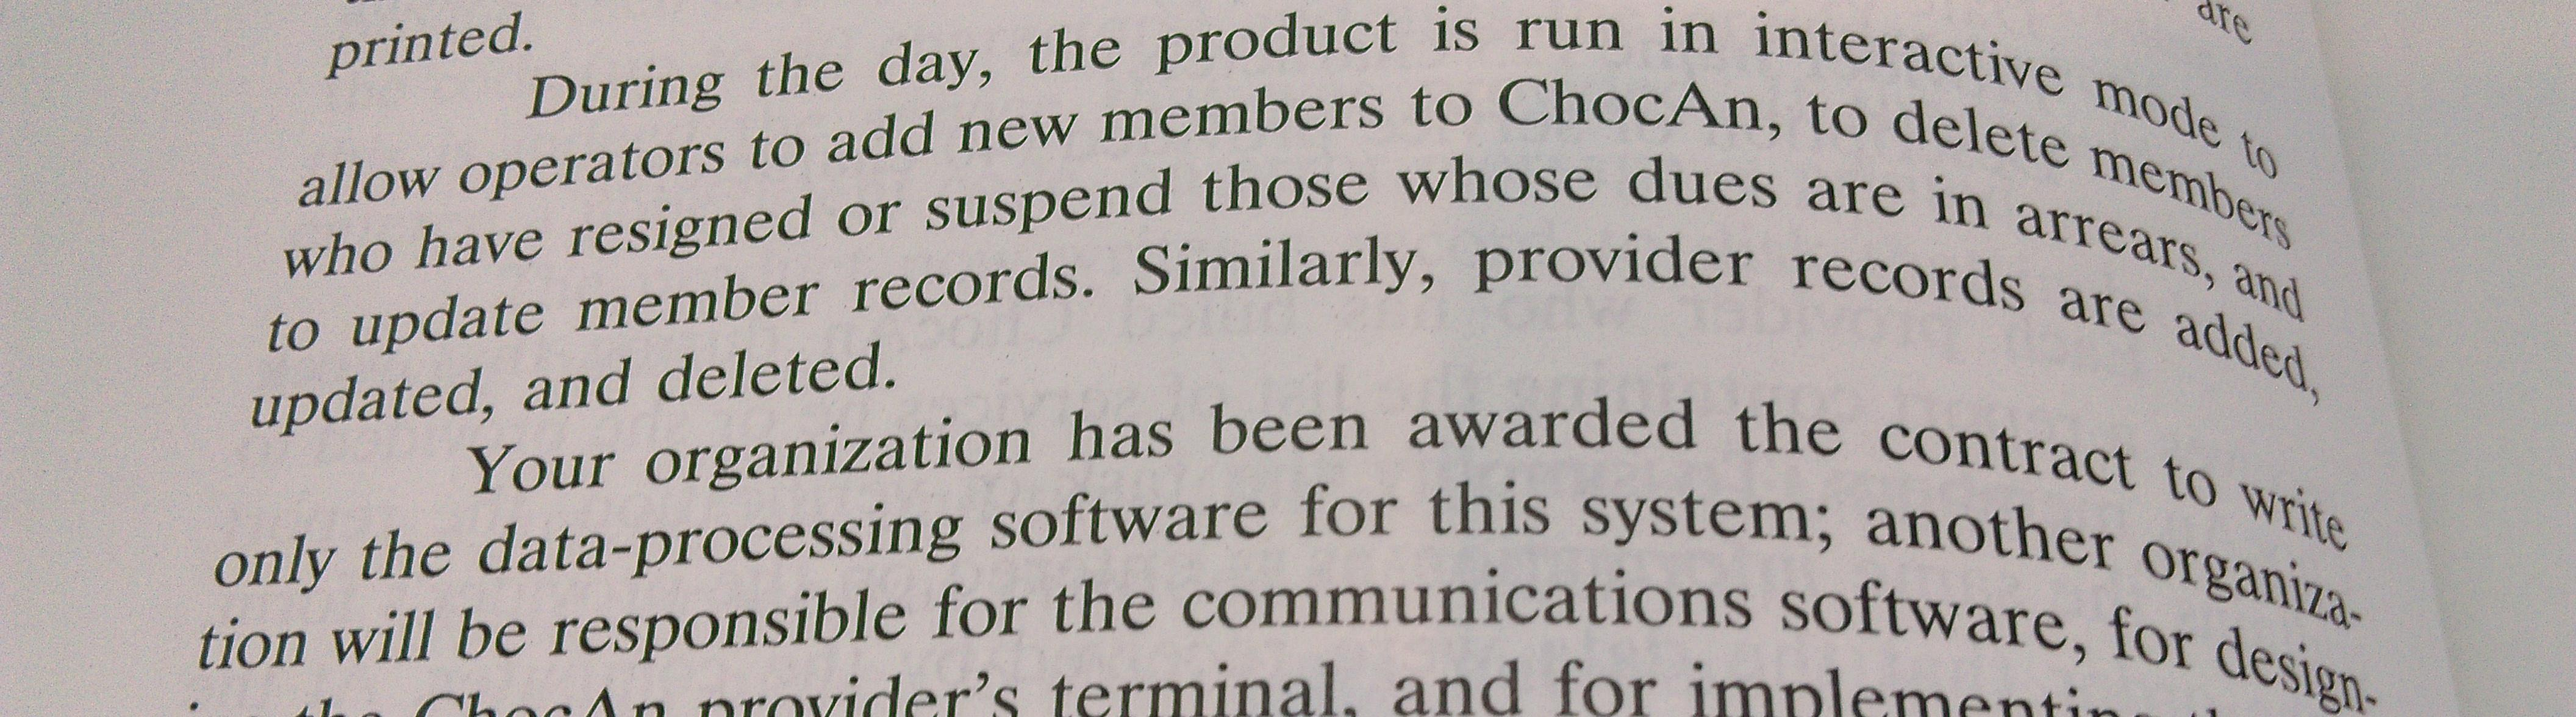
\includegraphics[width=\textwidth]{images/book-example-03.jpg}
    \caption{Primjer slike sadržaja iz knjige.}
    \label{fig:book-example-03}
\end{figure}
\end{frame}
\begin{frame}
\frametitle{Skup podataka za ispitivanje}
\framesubtitle{Slike (2)}
\begin{figure}[htb]
    \centering
    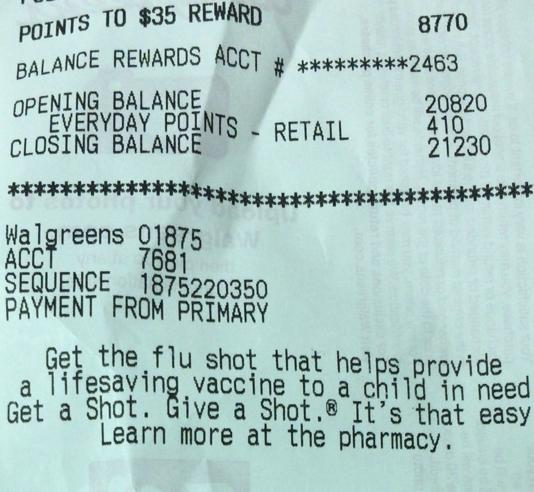
\includegraphics[width=7cm]{images/receipt-example-04.jpg}
    \caption{Primjer slike računa iz trgovine.}
    \label{fig:receipt-example-04}
\end{figure}
\end{frame}
\begin{frame}
\frametitle{Skup podataka za ispitivanje}
\framesubtitle{Slike (3)}
\begin{figure}[htb]
    \centering
    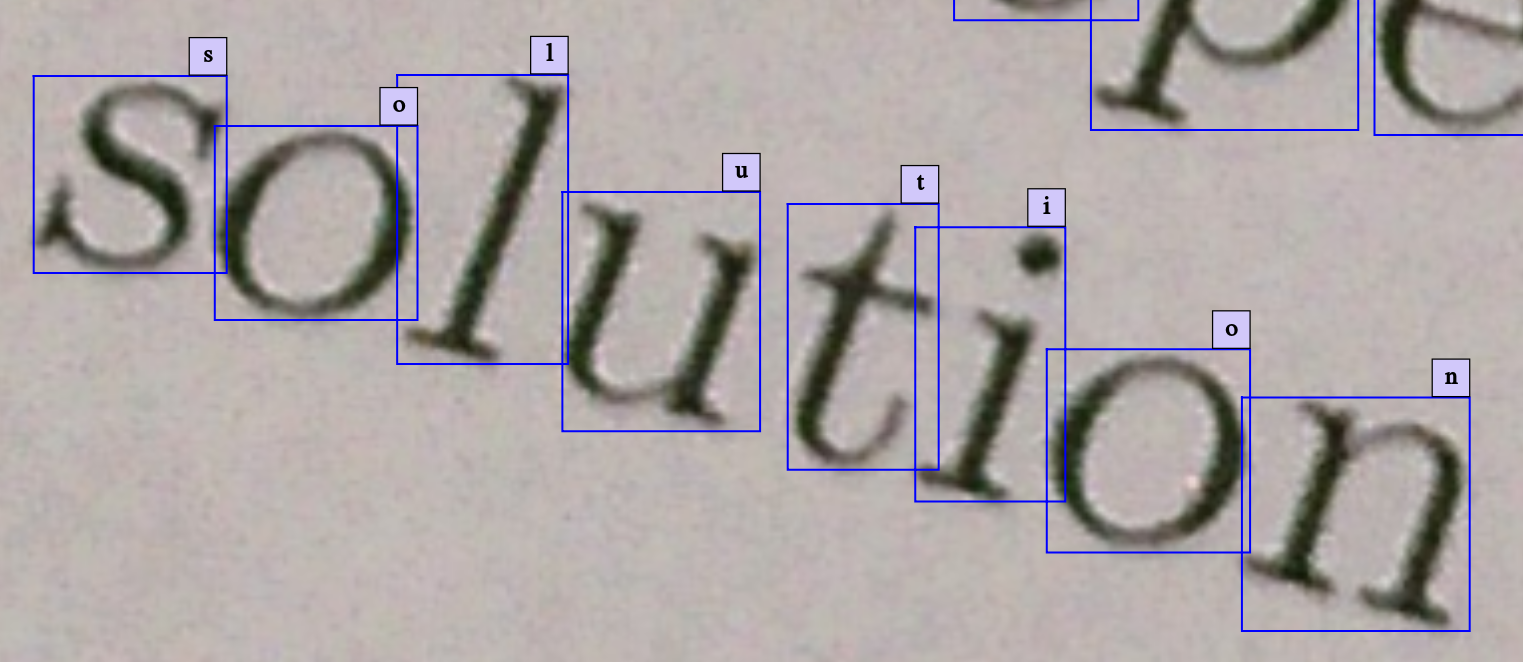
\includegraphics[width=\textwidth]{images/book-example-04.png}
    \caption{Primjer slike s ukošenim tekstom.}
    \label{fig:book-example-04}
\end{figure}
\end{frame}
\begin{frame}
\frametitle{Skup podataka za ispitivanje}
\framesubtitle{Ulazne datoteke}
\begin{itemize}
    \item Slike \textbf{ne predstavljaju} ulaz u sustav za određivanje strukture teksta.
    \item Ulazne datoteke u formatu JSON predstavljaju nestrukturirani OCR-rezultat.
    \item Za svaki znak poznate su sljedeće informacije:
    \begin{itemize}
        \item $x$ - horizontalna pozicija gornjeg lijevog kuta,
        \item $y$ - vertikalna pozicija gornjeg lijevog kuta,
        \item $width$ - širina,
        \item $height$ - visina i
        \item $value$ - Unicode vrijednost.
    \end{itemize}
\end{itemize}
\end{frame}
\begin{frame}[fragile]
\frametitle{Skup podataka za ispitivanje}
\framesubtitle{Očekivane izlazne datoteke}
\begin{lstlisting}[
    caption={Ispravni tekstualni sadržaj slike \protect\ref{fig:receipt-example-04}.},
    firstnumber=1,
    label={lst:txt-result-04}
]
POINTS TO $35 REWARD 8770
BALANCE REWARDS ACCT # *********2463
OPENING BALANCE 20820
EVERYDAY POINTS - RETAIL 410
CLOSING BALANCE 21230
*****************************************
Walgreens 01875
ACCT 7681
SEQUENCE 1875220350
PAYMENT FROM PRIMARY
Get the flu shot that helps provide
a lifesaving vaccine to a child in need
Get a Shot. Give a Shot.® It's that easy
Learn more at the pharmacy.
\end{lstlisting}
\end{frame}


\subsection{Korištenje skupa podataka za ispitivanje}
\begin{frame}
\frametitle{Skup podataka za ispitivanje}
\framesubtitle{Korištenje skupa podataka za ispitivanje (1)}
\begin{figure}[htb]
    \centering
    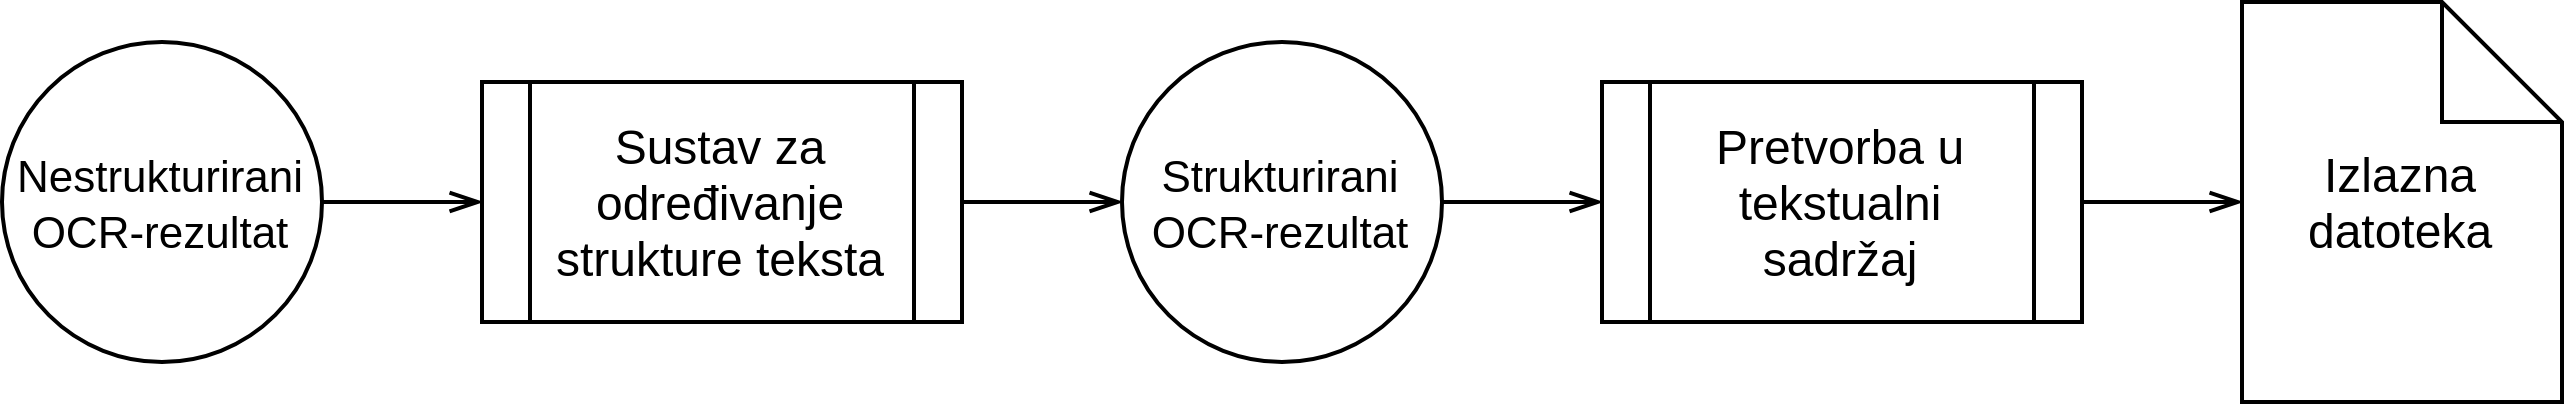
\includegraphics[width=\textwidth]{images/sustav-02.png}
    \caption{Postupak dobivanja izlazne datoteke iz strukturiranog OCR-rezultata.}
    \label{fig:sustav-02}
\end{figure}
\end{frame}
\begin{frame}[fragile]
\frametitle{Skup podataka za ispitivanje}
\framesubtitle{Korištenje skupa podataka za ispitivanje (2)}
\begin{lstlisting}[
    caption={Pseudokôd algoritma za ispis OCR-rezultata.},
    label={lst:ocr-result-to-txt},
    morekeywords={def,for,end,if,else,return},
    firstnumber=1,
    xleftmargin=.1\textwidth,
    xrightmargin=.1\textwidth
]
def ispisi(ocrRezultat)
  for linija u ocrRezultat.linije
    for znak u linija
      print(znak.value)
    end
    print("\n")
  end
end
\end{lstlisting}
\end{frame}

\section{Algoritmi za određivanje strukture teksta}
\begin{frame}
\frametitle{Algoritmi za određivanje strukture teksta}
\framesubtitle{Komponente sustava za određivanje strukture teksta}
\begin{figure}[htb]
    \centering
    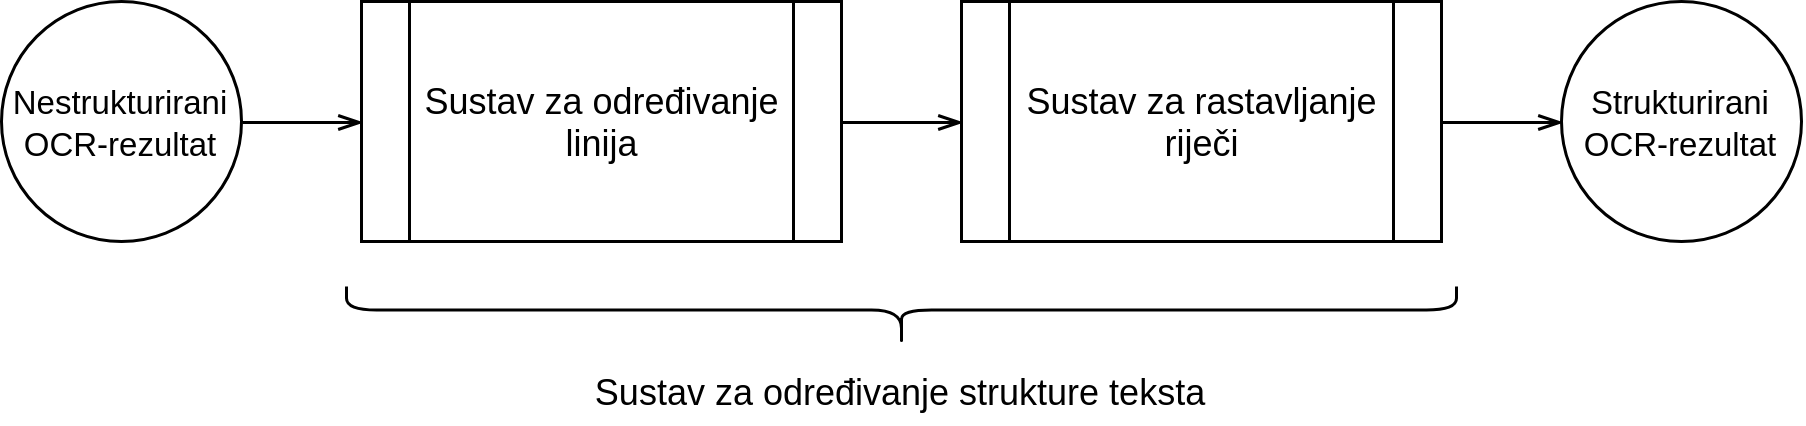
\includegraphics[width=\textwidth]{images/sustav-03.png}
    \caption{Komponente sustava za određivanje strukture teksta.}
    \label{fig:sustav-03}
\end{figure}
\end{frame}

\subsection{Algoritmi za određivanje linija}
\begin{frame}
\frametitle{Algoritmi za određivanje strukture teksta}
\framesubtitle{Algoritmi za određivanje linija}
\begin{figure}[htb]
    \centering
    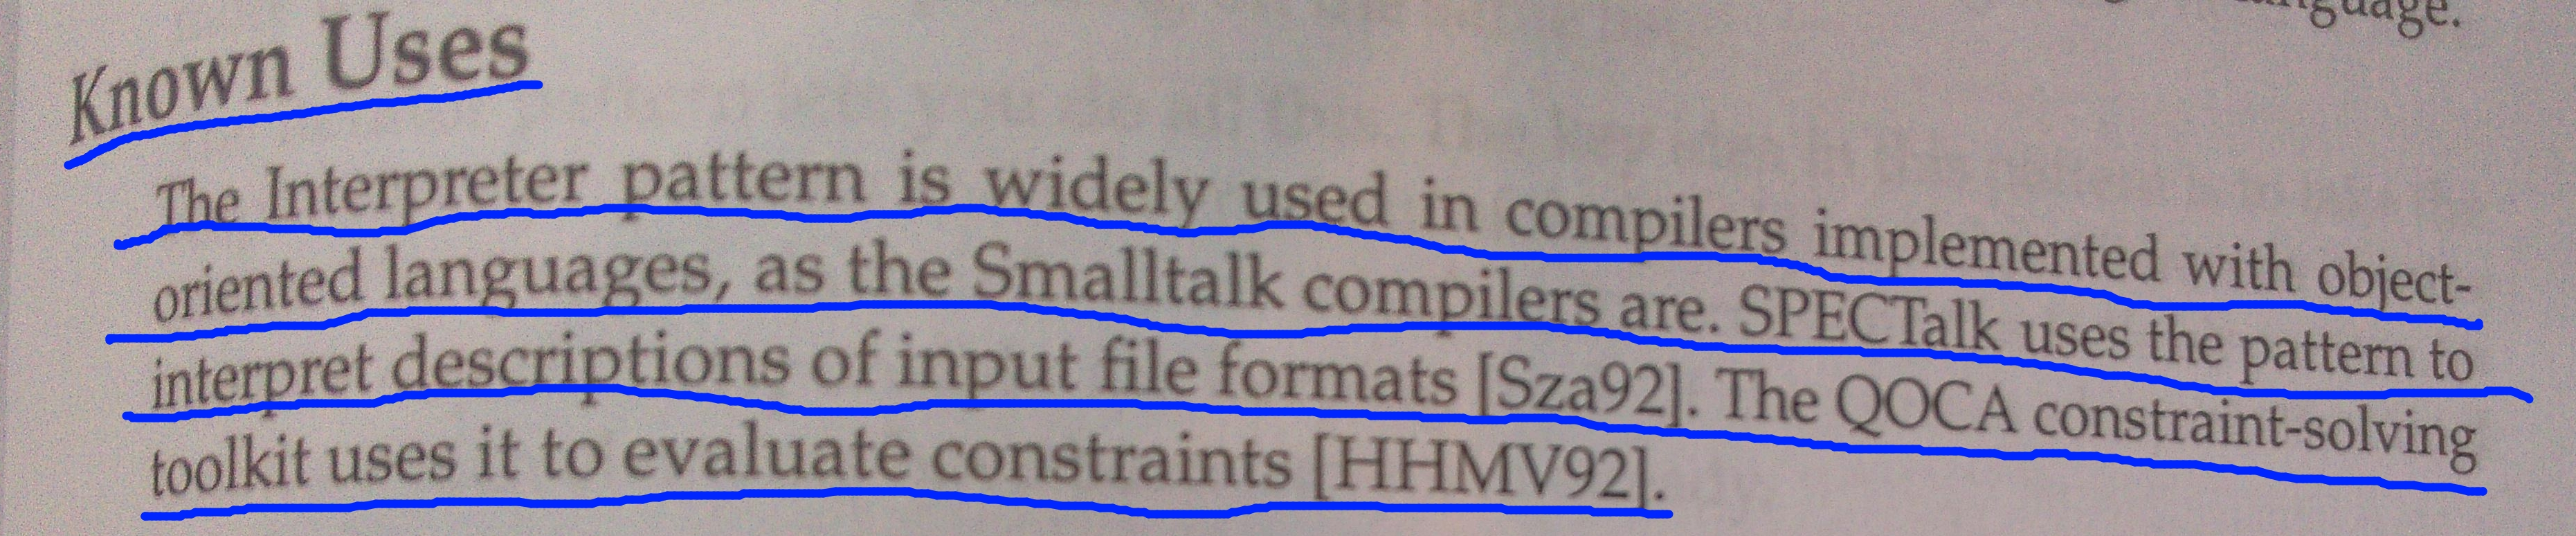
\includegraphics[width=\textwidth]{images/line-segmentation-01.jpg}
    \caption{Vizualizacija detektiranih linija u sadržaju iz knjiga.}
    \label{fig:line-segmentation-01}
\end{figure}
\end{frame}
\begin{frame}
\frametitle{Algoritmi za određivanje linija}
\framesubtitle{Algoritam temeljen na maksimalnom preklapanju znakova (1)}
\begin{itemize}
    \item Temelji se na pretpostavci da dva susjedna znaka koje se nalaze u istoj
          liniji ostvaruju maksimalno vertikalno preklapanje.
    \item Vertikalno preklapanje dva znaka definira se izrazom:
\end{itemize}
\
\begin{equation}
\label{eq:overlap}
\textit{overlap}(A, B) =
\frac{\max(0, \min( A_y + A_h, B_y + B_h ) - \max( A_y, B_y ))}{\min(A_h, B_h)}
\end{equation}
\begin{figure}[htb]
    \centering
    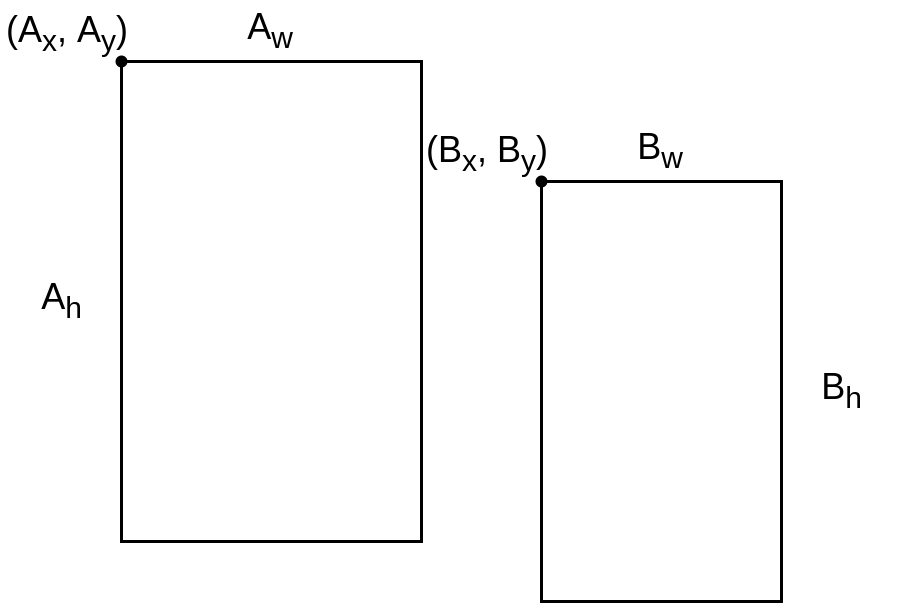
\includegraphics[height=3cm]{images/chars-01.png}
    \caption{Omeđujući pravokutnici znakova.}
    \label{fig:chars-01}
\end{figure}
\end{frame}
\begin{frame}
\frametitle{Algoritmi za određivanje linija}
\framesubtitle{Algoritam temeljen na maksimalnom preklapanju znakova (2)}
\begin{itemize}
    \item Algoritam izgrađuje linije.
    \item Na početku, algoritam uzlazno sortira sve znakove po~horizontalnoj~$x$~vrijednost.
    \item Promatrani znak pridružuje se onoj liniji s kojom ostvari~maksimalno~preklapanje:
\end{itemize}
\
\begin{equation}
\label{eq:overlap-01}
l_{max} = \argmax_{l \in L}\left\{\textit{overlap}(A, l_{-1})\right\}
\end{equation}
\begin{itemize}
    \item Za preklapanje vrijednosti 0, u skup $L$ dodaje se nova linija i
          promatrani znak postaje početak te linije.
\end{itemize}
\end{frame}
\begin{frame}
\frametitle{Algoritmi za određivanje linija}
\framesubtitle{Algoritam temeljen na maksimalnom preklapanju znakova (3)}
\begin{itemize}
\item Ponekad je poželjno izmjeriti preklapanje ne samo sa zadnjim znakom u liniji,
nego i sa zadnjih nekoliko znakova:
\end{itemize}
\
\begin{equation}
\label{eq:overlap-02}
l_{max} = \argmax_{l \in L,\ i \in [1, \min(|l|, c_1)]}\left\{\textit{overlap}
(A, l_{-i})\right\}
\end{equation}
\begin{figure}[htb]
    \centering
    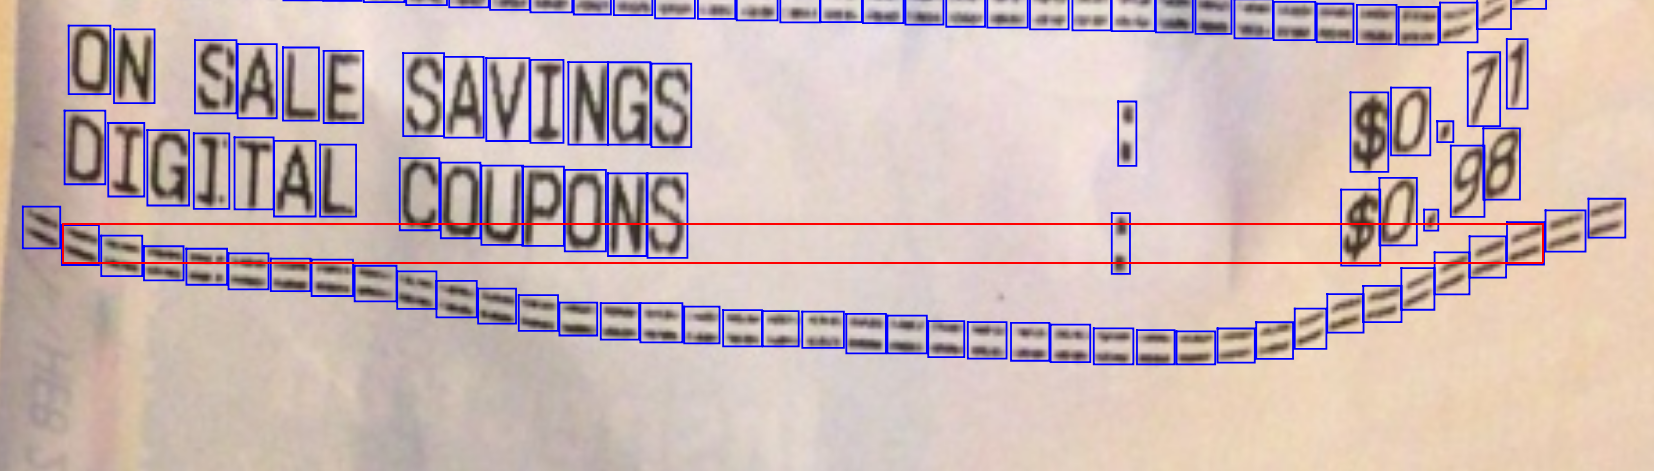
\includegraphics[width=.9\textwidth]{images/aligner-01.png}
    \caption{Valovite linije otežavaju određivanje linija.}
    \label{fig:aligner-01}
\end{figure}
\end{frame}
\begin{frame}
\frametitle{Algoritmi za određivanje linija}
\framesubtitle{Algoritam temeljen na maksimalnom preklapanju znakova (4)}
\begin{itemize}
    \item Uvodi se dodatan uvijet koji će odlučiti hoće
    li promatrani znak pripasti liniji s kojom ostvaruje maksimalno preklapanje:
\end{itemize}
\
\begin{equation}
\label{eq:overlap-03}
\max_{i \in [1, \min(|l_{max}|, c_1)]}\left\{\textit{overlap}(A, l_{max_{-i}})
\right\} > c_2
\end{equation}
\begin{figure}[htb]
    \centering
    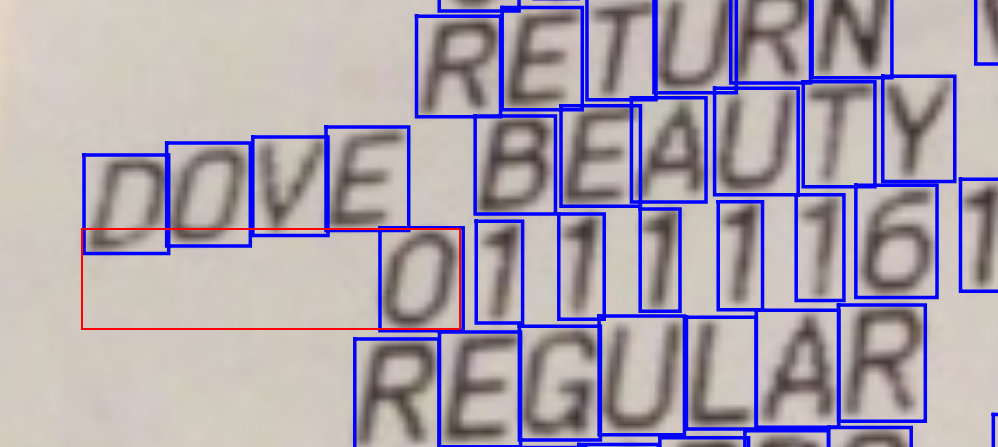
\includegraphics[width=.7\textwidth]{images/overlap-01.png}
    \caption{Preklapanje početaka dviju linija.}
    \label{fig:overlap-01}
\end{figure}
\end{frame}
\begin{frame}
\frametitle{Algoritmi za određivanje linija}
\framesubtitle{Algoritam temeljen na maksimalnom preklapanju znakova (5)}
\begin{itemize}
    \item Za rješavanje problema lažnog pozitivnog preklapanja definiraju se dvije
          funkcije:
\end{itemize}
\begin{align}
    f_1(x) &= \frac{1}{1 + c_3 \cdot x} \\[10pt]
    f_2(x) &= 1 + \frac{c_4 \cdot x}{1 + c_4 \cdot x}
\end{align}
\begin{figure}[htb]
    \centering
    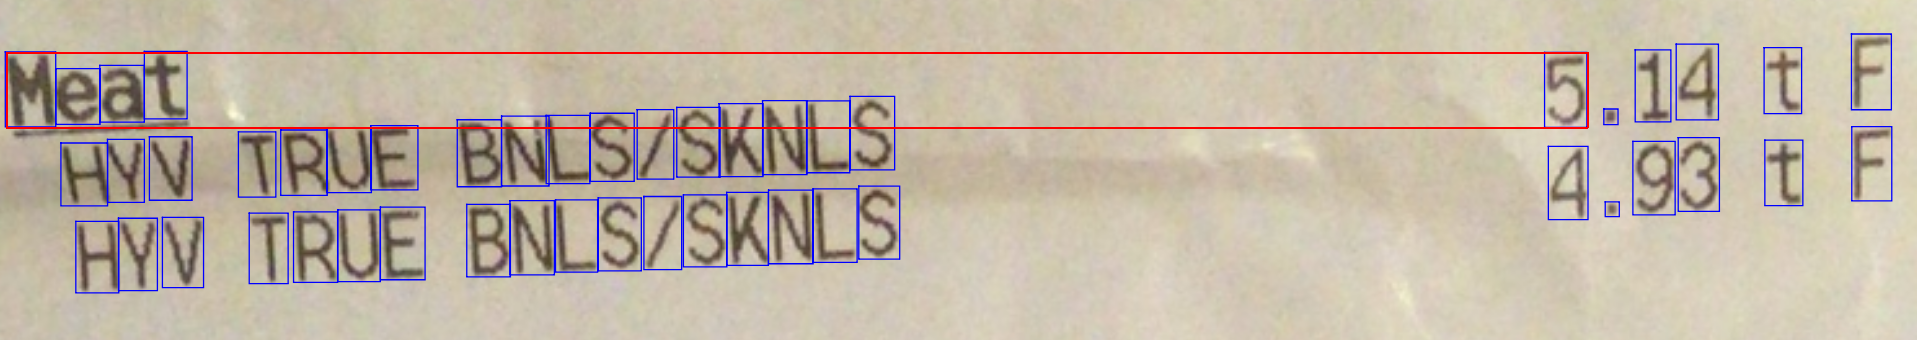
\includegraphics[width=\textwidth]{images/overlap-02.png}
    \caption{Lažno pozitivno preklapanje.}
    \label{fig:overlap-02}
\end{figure}
\end{frame}
\begin{frame}
\frametitle{Algoritmi za određivanje linija}
\framesubtitle{Algoritam temeljen na maksimalnom preklapanju znakova (6)}
\begin{figure}[htb]
    \centering
    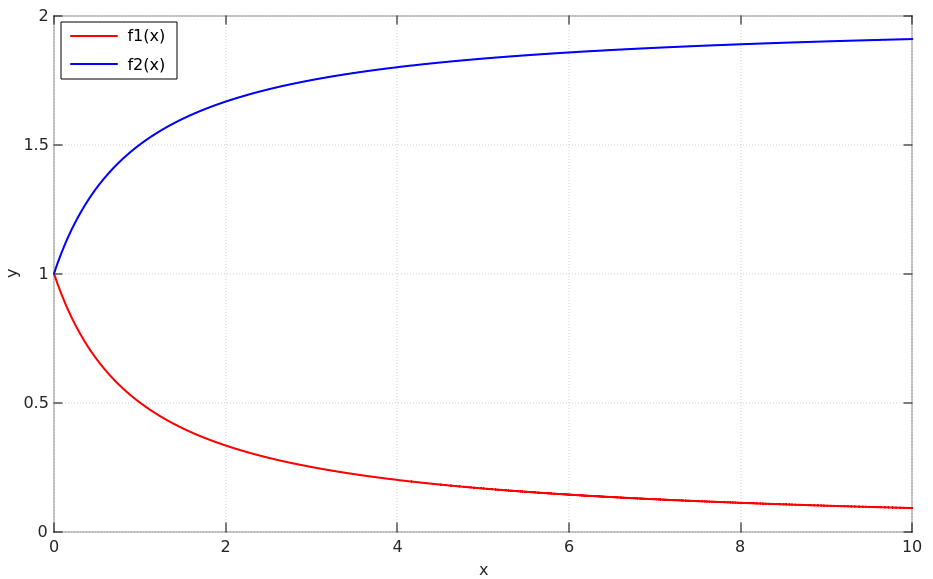
\includegraphics[width=.8\textwidth]{images/function-01.png}
    \caption{Grafovi funkcije $f_1$ (crveno) i funkcije $f_2$ (plavo).}
    \label{fig:function-01}
\end{figure}
\end{frame}
\begin{frame}
\frametitle{Algoritmi za određivanje linija}
\framesubtitle{Algoritam temeljen na maksimalnom preklapanju znakova (7)}
Iterirajući po skupu $L$ računamo preklapanje sa svakom linijom.
Neka znak u jednom trenutku pripada liniji $l$ s kojom ostvaruje preklapanje $p_l$.
U idućem koraku iteracije računamo preklapanje znaka s linijom $k$.
Postavljamo nove uvjete za pridruživanje znaka liniji $k$.

\

Znak će pripasti liniji $k$ ako je zadnji znak linije $k$ bliži promatranom znaku
od zadnjeg znaka linije $l$ i ako vrijedi:
\begin{equation}
p_k > p_l \cdot f_1(\hat{d_l}(l_{-1},k_{-1}))
\end{equation}

Znak će pripasti liniji $k$ ako je zadnji znak linije $k$ dalji od promatranog znaka
nego zadnji znak linije $l$ i ako vrijedi:
\begin{equation}
p_k > p_l \cdot f_2(\hat{d_l}(l_{-1},k_{-1}))
\end{equation}
\end{frame}

\subsection{Algoritmi za rastavljanje riječi}
\begin{frame}
\frametitle{Algoritmi za određivanje strukture teksta}
\framesubtitle{Algoritmi za rastavljanje riječi}
\begin{itemize}
    \item Na ulaz primaju OCR-rezultat s grupiranim linijama.
    \item Trebaju ubaciti znakove bjeline između znakova za koje smatra
          da su završetak prethodne i početak iduće riječi.
    \item Razvijena su tri algoritma za rastavljanje riječi:
    \begin{itemize}
        \item algoritam temeljen na prosječnoj širini znaka,
        \item algoritam temeljen na prosječnoj relativnoj udaljenosti i
        \item algoritam temeljen na prosječnoj udaljenosti centara.
    \end{itemize}
\end{itemize}
\begin{figure}[htb]
    \centering
    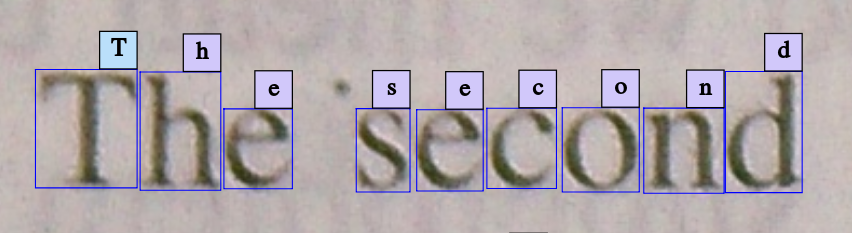
\includegraphics[width=.8\textwidth]{images/book-example-02.png}
    \caption{Linija s dvije riječi.}
    \label{fig:book-example-02}
\end{figure}
\end{frame}
\begin{frame}
\frametitle{Algoritmi za rastavljanje riječi}
\framesubtitle{Algoritam temeljen na prosječnoj širini znaka}
\begin{itemize}
    \item Najjednostavniji razvijeni algoritam.
    \item Temelji se na pretpostavci da je širina razmaka između riječi
          proporcionalna prosječnoj širini znakova u promatranoj liniji.
    \item Prosječna širina znaka u liniji $l$ računa se na sljedeći način:
\end{itemize}
\begin{equation}
\overline{w_l} = \frac{\mathlarger{\sum}\limits_{A \in l} A_w}{|l|}
\end{equation}
\begin{itemize}
    \item Algoritam ubacuje znak bjeline između znakova $A$ i $B$ ako vrijedi:
\end{itemize}
\begin{equation}
\label{eq:condition-01}
d(A, B) > \overline{w_l} \cdot c_1
\end{equation}
\end{frame}
\begin{frame}
\frametitle{Algoritmi za rastavljanje riječi}
\framesubtitle{Algoritam temeljen na prosječnoj relativnoj udaljenosti (1)}
\begin{itemize}
    \item Temelji se na pretpostavci da je udaljenost znaka $A$ s vrijednosti
          \engl{value} $A_v$ proporcionalna prosječnoj udaljenosti koju svi
          znakovi s vrijednost $A_v$ ostvaruju sa svojim susjedima.
\end{itemize}
\end{frame}
\begin{frame}
\frametitle{Algoritmi za rastavljanje riječi}
\framesubtitle{Algoritam temeljen na prosječnoj relativnoj udaljenosti (2)}
\begin{figure}[htb]
    \centering
    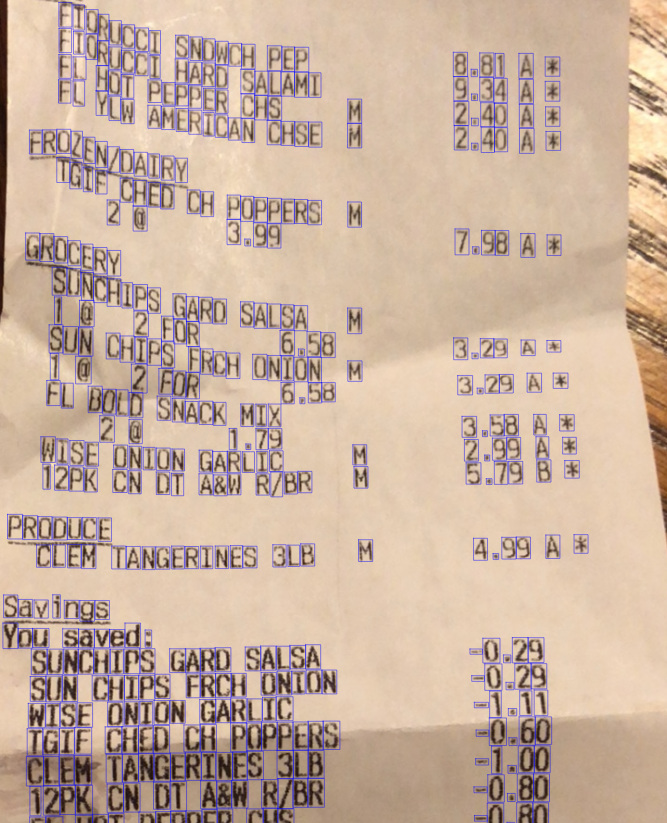
\includegraphics[height=.73\textheight]{images/receipt-example-03.png}
    \caption{Slika računa iz trgovine.}
    \label{fig:receipt-example-03}
\end{figure}
\end{frame}
\begin{frame}
\frametitle{Algoritmi za rastavljanje riječi}
\framesubtitle{Algoritam temeljen na prosječnoj relativnoj udaljenosti (3)}
\begin{itemize}
    \item Skup svih susjeda znaka $A$ definiramo kao skup svih znakova $B$ koji
          su različiti od $A$, koji pripadaju istoj liniji kao i $A$, i za koje
          vrijedi:
    \begin{equation}
    \hat{d_c}(A, B) < c_1 \texttt{.}
    \end{equation}
    \item Skup svih susjeda vrijednosti $v$ definiramo kao:
    \begin{equation}
    s(v) = \bigcup\limits_{A \in C}\left\{S(A) \vert A_v = v\right\}
    \end{equation}
    \item Prosječna udaljenost između znakova $A$, za koje vrijedi
          $A_v = v$, računa se na sljedeći način:
    \begin{equation}
    \label{eq:relative-distance-02}
    \overline{d_c}(v) =
    \frac{
        \mathlarger{\sum}\limits_{B \in C,\ B_v = v}
        \Bigg[
        \mathlarger{\sum}\limits_{D \in S(B)} d_c(B, D)
        \Bigg]
    }{|s(v)|}
    \end{equation}
\end{itemize}
\end{frame}
\begin{frame}
\frametitle{Algoritmi za rastavljanje riječi}
\framesubtitle{Algoritam temeljen na prosječnoj relativnoj udaljenosti (4)}
\begin{itemize}
    \item Algoritam ubacuje znak bjeline između znakova $A$ i $B$ ako vrijedi:
\end{itemize}
\begin{equation}
\label{eq:relative-distance-03}
    d_c(A, B) > \overline{d_c}(A_v) \cdot c_2 \quad \lor \quad
    d_c(A, B) > \overline{d_c}(B_v) \cdot c_2
\end{equation}
\end{frame}
\begin{frame}
\frametitle{Algoritmi za rastavljanje riječi}
\framesubtitle{Algoritam temeljen na prosječnoj udaljenosti centara (1)}
\begin{itemize}
    \item Temelji se na pretpostavci da je širina razmaka između riječi proporcionalna
          s prosječnom udaljenosti centara između susjednih znakova.
    \item Skup svih susjeda znaka $A$ definira se kao i u algoritmu temeljenom
          na prosječnoj relativnoj udaljenosti.
    \item Prosječna udaljenost centara između susjednih znakova u liniji
          $l$ definira se na sljedeći način:
    \begin{equation}
    \overline{d_c}(l) =
    \frac{
        \mathlarger{\sum}\limits_{A \in l}
        \Bigg[
        \mathlarger{\sum}\limits_{B \in S(A)} d_c(A, B)
        \Bigg]
    }
    {\bigg|\bigcup\limits_{A \in l} S(A)\bigg|}
    \end{equation}
\end{itemize}
\end{frame}
\begin{frame}
\frametitle{Algoritmi za rastavljanje riječi}
\framesubtitle{Algoritam temeljen na prosječnoj udaljenosti centara (2)}
\begin{itemize}
\item Algoritam ubacuje znak bjeline između znakova $A$ i $B$ ako vrijedi:
\end{itemize}
\begin{equation}
d_c(A, B) > \overline{d_c}(l) \cdot c_2
\end{equation}
\end{frame}

\section{Mjere točnosti algoritama}
\section{Rezultati}
\section{Zaključak}

\begin{frame}
\frametitle{Literatura}
\bibliography{literatura}
\bibliographystyle{fer}
\end{frame}

\end{document}
